\section{Methodology}
\label{sec:methodology}

In this section we describe the proposed NDN model in detail. We start with 
an overview, setting the notation and crudely establishing its relation 
with nonlinear dynamical systems. We then continue with a detailed description 
of each model component and related procedures.

\subsection{Overview}
\label{subsec:meth-overview}

We consider a conceptual NDN network composed by three main types of 
entities: (1) 
$|R|$ NDN routers\footnote{Here we use the notation $|E|$ to 
represent the number of elements of type $E$.} $R_r$, $r = \{1,2,...,|R|\}$, 
organized in some type of topology (e.g. cascade, tree, etc.); (2) a set of 
$|C|$ clients $C_c$, $c = \{1,2,...,|C|\}$; and a single 
content server $S$, holding $|O|$ different content objects $O_o$, 
$o = \{1,2,...,|O|\}$ (e.g. $|O|$ different photos).\shortvertbreak

Clients issue requests for content objects $O_o$, i.e. Interest packets $i_{O_o}$, which 
are propagated through NDN routers towards the content server $S$, and 
eventually followed by Data packets 
$d_{O_o}$, containing the requested content object. We represent the 
elementary set of signals fed to\slash read from the inputs\slash outputs of the 
aforementioned basic 
entities, at some discrete time $n$, as a $2\,|O| \times 1 $ vector in the form

\begin{equation}
    \textbf{v}[n] = \begin{bmatrix}  i_{O_1}         \\ 
                            i_{O_2}         \\ 
                             ...            \\ 
                            i_{O_{|O|}}     \\ 
                            d_{O_1}         \\ 
                            d_{O_2}         \\ 
                             ...            \\ 
                            d_{O_{|O|}}     \\ \end{bmatrix}
    \label{eq:signal}
\end{equation}\shortvertbreak

Each component $i_{O_o}$ or $d_{O_o}$ may assume an integer value, i.e. $i_{O_o}, d_{O_o} \in \mathbb{N}_0 = \{0, 1, 2, ... \}$, 
representing the absence (in case of $i_{O_o}, d_{O_o} = 0$) or presence (in case of $i_{O_o}, d_{O_o} > 0$) of an 
Interest\slash Data packet, at a given discrete time $n$. E.g. considering a setting 
with $|O| = 2$ content objects, a value of \textbf{x} corresponding to the presence 
of two Interests for content $O_1$ and one Data packet for $O_2$ (with the absence 
for the remaining components) would be encoded as

\begin{equation}
    \textbf{v}[n] = \begin{bmatrix}     2   \\ 
                                        0   \\ 
                                        0   \\ 
                                        1   \\ \end{bmatrix}
    \label{eq:signal-eg}
\end{equation}\shortvertbreak

With this 
representation, we capture situations in which a network 
entity may simultaneously receive\slash issue any Interest or Data packet at 
its input\slash output. Our models for NDN routers, clients or servers can be 
seen as nonlinear dynamical subsystems, accepting inputs \textbf{u} and producing 
outputs \textbf{y}, in the form shown in~\ref{eq:signal} 
and~\ref{eq:signal-eg}. Furthermore, each one of these subsystems exhibits one or 
more types of state \textbf{x} (e.g. the composition of a Content Store or a Pending 
Interest Table), which evolves according to nonlinear dynamics $\mathcal{H}$, 
driven by \textbf{u} and the current state \textbf{x}:

\begin{equation}
    \textbf{x}[n + 1] = \mathcal{H}(\textbf{x}[n],\textbf{u}[n])
    \label{eq:state}
\end{equation}%\shortvertbreak

Outputs \textbf{y} are nonlinearly related to some current state \textbf{x} and input \textbf{u}:

\begin{equation}
    \textbf{y}[n] = \mathcal{G}(\textbf{x}[n],\textbf{u}[n])
    \label{eq:outputs}
\end{equation}%\shortvertbreak

We also note that in some subsystems, namely at the clients $C$, the outputs 
\textbf{y} may include a stochastic component $w$ (e.g. in cases where Interest 
signals are randomly generated):

\begin{equation}
    \textbf{y}[n] = \mathcal{G}(\textbf{x}[n],\textbf{u}[n]) + w
    \label{eq:clients}
\end{equation}%\shortvertbreak

In the next subsections, we describe each one of the nonlinear subsystems in 
detail, including the types of state and associated nonlinear dynamics.

\subsection{NDN Router Model}
\label{subsec:meth-overview}

An NDN router is the central entity of the presented model, acting 
as the main agent of NDN's forwarding engine. It is also the more complex entity, 
including a set of submodules, already 
mentioned in Section~\ref{sec:ndn}: (1) the Pending Interest Table (PIT); (2) 
the Content Store (CS); and (3) the Forward Information Base (FIB). We first 
provide an overview of our NDN router module, and then proceed with the description 
of each one of its submodules.\shortvertbreak

\begin{figure}[h!]

    \centering
    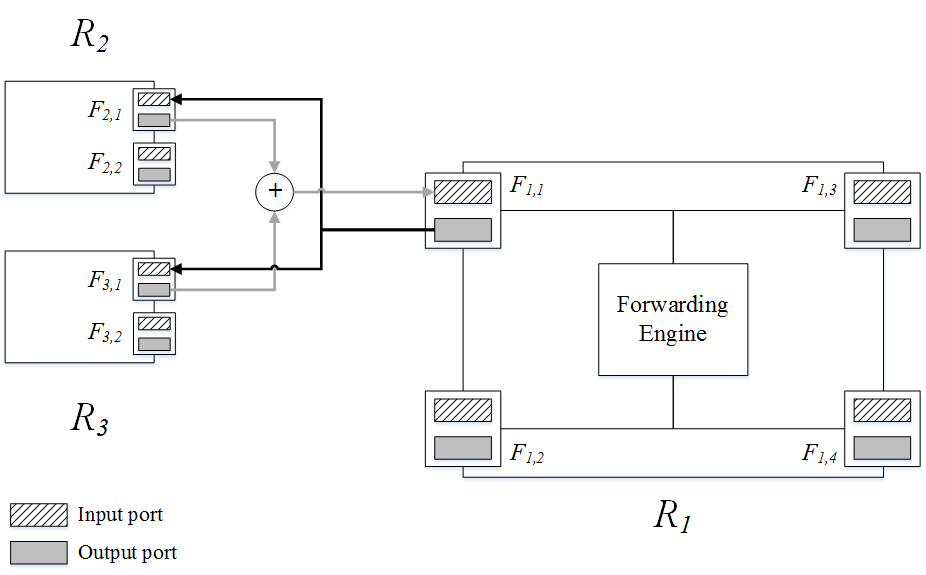
\includegraphics[width=0.40\textwidth]{figures/ndn-router-overview.png}
    \cprotect\caption{Graphical depiction of our NDN router model.}
    \label{fig:ndn-router-overview}

\end{figure}

Figure~\ref{fig:ndn-router-overview} provides a graphical description of the proposed 
router model. A router $R$ contains a set of $|F|$ interfaces $F$, used to interconnect 
it to other entities (e.g. some other router $R'$, a client $C$ or a server 
$S$). Each interface can subsequently be divided into one input and one output 
port, which `cross-connect' with the ports of the attached 
interfaces (see Figure~\ref{fig:ndn-router-overview}). We use the notation 
$F_{r,f,in}$ or $F_{r,f,out}$, to refer to the 
input\slash output ports of an interface with index $f$, of a router $R_r$\footnote{We 
adopt a flexible notation, sometimes referring to an interface as 
$F_{r,f}$ when there is no need to specify a particular port.}.\shortvertbreak

Taking Figure~\ref{fig:ndn-router-overview} as a supporting example, the act of 
forwarding some set of Interest\slash Data packets from a router $R_1$, 
over some interface $F_1$, is modeled by having $R_1$ fill $F_{1,1,out}$ with 
some set of signals \textbf{y}, following the encoding shown in 
Section~\ref{subsec:meth-overview}. Conversely, the act of receiving some set 
of Interest\slash Data packets is modeled by having routers $R_2$ and $R_3$ --- 
connected with $F_{1,1}$ via $F_{2,1}$ and $F_{3,1}$ --- fill $F_{2,1,in}$ and $F_{3,1,in}$ 
with \textbf{u} \footnote{In fact, this procedure can be extended to any network entity, let 
it be a router, a client or a server.}. As seen in Figure~\ref{fig:ndn-router-overview}, 
more than one entity may be connected to some interface, in which case the 
signals \textbf{y} originating from the interconnected interfaces' output ports, 
e.g. $F_{2,1,out}$ and $F_{3,1,out}$, are combined and summed at the other 
end's input port, e.g. $F_{1,1,in}$. While the use of interfaces and 
input\slash output ports may be seen as a case of over engineering, we argue 
it makes our model robust, highly modular and capable of supporting multiple 
network topologies.\shortvertbreak

\subsubsection{Pending Interest Table (PIT)}
\label{subsec:meth-pit}

In the same way that the FIB commands the forwarding of Interests, the PIT 
commands the forwarding of Data packets. The composition of the 
PIT is more dynamic than that of the FIB, being dependent on the flow of 
Interest and Data signals through the NDN router. We model the PIT as a 
$|O| \times |F|$ matrix in the form:

\begin{equation}
\textbf{PIT} = \begin{bmatrix} 1 & 0 & 0 & 0  \\ 
                1 & 0 & 0 & 0               \\ 
                0 & 1 & 0 & 0               \\ 
                0 & 1 & 0 & 0               \\ \end{bmatrix}
    \label{eq:pit}
\end{equation}\shortvertbreak

\textbf{PIT}\footnote{We use the form `PIT' for general references to the Pending 
Interest Table, and `\textbf{PIT}' when referring to its matrix form, as in~\ref{eq:pit}. 
This dual representation is extended to the FIB and CS.} entries 
$(o,f)$ are encoded as 0 or 1: if $(o,f) = 1$, Interests for content object 
$O_o$ have been previously received in interface $F_{r,f}$, and so Data 
packets $d_{O_o}$ shall be forwarded via $F_{r,f}$; on the other hand, 
if $(o,f) = 0$, $d_{O_o}$ should not be forwarded via that 
interface. The arrival of Interest and Data packets influences the composition of 
the PIT over time, each triggering special routines --- \textbf{PIT::updateOnInterest()} and 
\textbf{PIT::updateOnData()} --- shown below. We consider 
special $2\,|O| \times |F|$ matrices \textbf{U} and \textbf{Y}, corresponding to the concatenation of 
all the column vectors $\textbf{u}_{r,f}$ and $\textbf{y}_{r,f}$, i.e. the contents from the input and output ports 
of all the interfaces $F_{r,f}$, at some router $R_r$:

\begin{equation}
\textbf{U} = \begin{bmatrix} \textbf{u}_{r,1} & \textbf{u}_{r,2} & ... & \textbf{u}_{r,|F|} \end{bmatrix}
    \label{eq:a}
%\end{equation}\shortvertbreak
\end{equation}

\begin{equation}
\textbf{Y} = \begin{bmatrix} \textbf{y}_{r,1} & \textbf{y}_{r,2} & ... & \textbf{y}_{r,|F|} \end{bmatrix}
    \label{eq:b}
%\end{equation}\shortvertbreak
\end{equation}\shortvertbreak

\begin{algorithmic}[1]

\State \textbf{define} PIT::updateOnInterest(\textbf{U}):
\State
    \State $\textbf{U}' \leftarrow \textbf{U}(1:|O|,:)$
%    \State $\textbf{D} \leftarrow$ diag$(\neg(\textbf{PIT} \times \textbf{1}))$
    \State $\textbf{Y}'_i \leftarrow$ $\neg(\textbf{PIT} \times \textbf{1}^{|F|}) \ \& \ (\textbf{U}' \times \textbf{1}^{|F|})$
%    \State $\textbf{B} \leftarrow \textbf{D} \times \textbf{U}'$ 
    \State \textbf{PIT} $\leftarrow$ \textbf{PIT} $|$ $\textbf{U}'$ 
    \State \Return $\textbf{Y}'_i$

\end{algorithmic}\shortvertbreak

Upon the reception of Interest signals, i.e. $\textbf{U}'$ (the first $|O|$ rows 
of $\textbf{U}$), we first identify the content items $O_o$, or the row indexes $o$ of the 
\textbf{PIT}, for which there are \textbf{no} pending Interests (line 4). For 
convenience, we often recur to binary operations (negation `$\neg$', 
conjunction `$\&$', disjunction `$|$') over matrices: e.g. in line 4, after 
summing all columns of the \textbf{PIT}\footnote{We use the notation $\textbf{1}^{m}$ for the $m \times 1$
sum vector, i.e. $\textbf{1}^{m} = [1\,1\,...\,1]^{T}$.}, we negate the 
result, obtaining a binary encoded $|O| \times 1$ 
column vector which indicates the absence (encoded as  `1') and presence 
(encoded as `0') of pending Interests for some content object $O_o$. Still in 
line 4, we obtain a $|O| \times 1$ column vector, $\textbf{Y}'_i$, which encodes 
Interest signals which are not already stored and that the NDN router needs to forward upstream. This is 
accomplished by taking the logic AND, `$\&$', between $\neg(\textbf{PIT} \times \textbf{1}^{|F|})$ and 
$\textbf{U}'$. Note that even 
if $\textbf{U}'$ includes some $i_{O_o} > 1$, we only need to forward one Interest 
over the interfaces specified in the FIB, and so the binary encoding of $\textbf{Y}'_i$, 
resulting from the use of binary operations, neatly serves our purposes. 
In line 5, the 
contents of the \textbf{PIT} are updated by performing a logic OR, `$|$', with $\textbf{U}'$, so 
that it registers all the newly received 
Interest signals and their correspondence to interfaces. This last step is important, 
as it allows future Data packets to be forwarded downstream over the requesting 
interfaces.\shortvertbreak

\begin{algorithmic}[1]

\State \textbf{define} PIT::updateOnData($\textbf{U}$):
\State
    \State $\textbf{U}' \leftarrow \textbf{U}(|O|+1:2\,|O|,:)$
    \State $\textbf{G} \leftarrow (\textbf{U}' \times \textbf{1}^{|F|}) \times {\textbf{1}^{|F|}}^{T}$
%    \State $\textbf{D} \leftarrow \textbf{U}' \times \textbf{1}$
    \State $\textbf{Y}_d \leftarrow$ $\textbf{PIT} \ \& \ \textbf{G}$
    \State \textbf{PIT} $\leftarrow$ $\textbf{PIT} \ \& \ \neg\textbf{G}$ 
    \State \Return $\textbf{Y}_d$

\end{algorithmic}\shortvertbreak

%With the explanation given above for the \textbf{PIT::updateOnInterest()} routine, 
%the understanding of \textbf{PIT::updateOnData()} is left to the reader. 
Note that 
the objective of PIT::updateOnData() is the reverse operation of PIT::updateOnInterest(), i.e. forwarding Data 
packets over the interfaces for which there is a registered Interest in the \textbf{PIT}, with 
the result encoded in matrix $\textbf{Y}_d$. $\textbf{G}$ consists in a $|O| \times |F|$ matrix, which expands the single-column 
vector $\textbf{U}' \times \textbf{1}^{|F|}$ to $|F|$ columns (line 4), making it ready 
for the subsequent AND (`\&') operations (lines 5 and 6). The final 
step of the operation (line 6) consists in erasing 
all Interest registrations which have been successfully attended.\shortvertbreak

As a final remark, we can now identify the \textbf{PIT} as one form of state 
\textbf{x}, which is driven by the nonlinear dynamics specified on the 
PIT::updateOnInterest() and PIT::updateOnData() routines (lines 5 and 6, respectively). 
Furthermore, both routines also contribute to the generation of outputs, 
in the form of matrices $\textbf{Y}_d$ and $\textbf{Y}'_i$.\shortvertbreak

\subsubsection{Content Store (CS)}
\label{subsec:meth-cs}

We model the Content Store (CS), i.e. the NDN router's cache, as an $|O| 
\times |P|$ matrix, in which $|P|$ is the size of the CS, i.e. maximum 
number of content objects it is able to accommodate at any given point in time. 
We use $P$ to represent a position or slot in the CS, which is able to hold a single 
content object $O_o$ (here we do not consider a notion of content object size, 
an object always fits in a slot $P$). E.g. in~\ref{eq:cs} we show the encoding 
of the \textbf{CS} for $R_1$ in Figure~\ref{fig:fib-topo}, with $|P| = 2$, 
which is shown to contain content objects $O_2$ and $O_4$\footnote{Usually, 
we consider $|P| << |O|$.}.

\begin{equation}
\textbf{CS} = \begin{bmatrix} 0 & 0             \\ 
                1 & 0                           \\ 
                0 & 1                           \\ 
                0 & 0                           \\ \end{bmatrix}
    \label{eq:cs}
\end{equation}\shortvertbreak

Again, we follow a binary encoding, using $(o, p) = 1$ to indicate the 
presence of content $O_o$ at slot $P_p$, and $(o, p) = 0$ as an indication of 
its absence. Each slot is assigned a different integer 
index, i.e. $P_p$, with $p = \{1, 2, ..., |P|\}$, which express the idea of `cache levels': 
$O_o$, occupying slot $P_2$, is at the 2\textsuperscript{nd} 
(highest) position of the \textbf{CS}. $P_1$ is usually interpreted as the `highest' 
level, and $P_{|P|}$ the `lowest', nevertheless the meaning is of the `levels' 
is often dependent on the cache algorithm implemented by the CS.\shortvertbreak
%In fact, we 
%model a CS as having a general behavior (presented in this section), and a specific 
%behavior, which depends on the cache algorithm the CS implements. We discuss cache 
%algorithms in Section~\ref{subsec:meth-caching-algs}.\shortvertbreak

Note that \textbf{CS} must obey a set of constraints, since (1) 
each slot can only hold a single content object, and (2) it is inefficient for 
the \textbf{CS} to hold multiple copies of a content $O_o$. Specifically, the 
conditions for the validity of \textbf{CS} are:

\begin{equation}
    \sum_{o=1}^{|O|} \textbf{CS}_{o,p} \le 1 \quad \forall \ p \in {1, 2, ..., |P|}
    \label{eq:cs-constraints-1}
\end{equation}

\begin{equation}
    \sum_{p=1}^{|P|} \textbf{CS}_{o,p} \le 1 \quad \forall \ o \in {1, 2, ..., |O|}
    \label{eq:cs-constraints-2}
\end{equation}

Similarly to the PIT, the operations related to the CS are implemented by two 
routines: \textbf{CS::updateOnInterest()} and \textbf{CS::updateOnData()}. While 
the behavior of CS::updateOnData() is specific to a particular cache 
algorithm (see Section~\ref{subsec:meth-caching-algs}), that of CS::updateOnInterest() 
is rather general, consisting in the generation of a pair of $|O| \times |F|$ 
matrices, $[\textbf{Y}_h, \textbf{R}]$. In short, $\textbf{Y}_h$ encodes 
the Data packets for which there are cache hits, already assigned to the 
appropriate interface columns; and $\textbf{R}$ encodes all the Interest signals 
for which there were no cache hits\footnote{Due to space constraints, we do not 
show the algorithm of CS::updateOnInterest(), which can nevertheless be 
consulted in \url{github.com/adamiaonr/mtsp-project}.}.\shortvertbreak

Again, \textbf{CS} may be seen as the other form of state in the NDN router 
subsystem, driven by the nonlinear dynamics specified by each different 
cache algorithm. Furthermore, the CS::updateOnInterest() 
routine, common to all caching policies, contributes to the generation of the 
output matrix \textbf{Y} via $\textbf{Y}_h$.\shortvertbreak

\subsubsection{Forwarding Information Base (FIB)}
\label{subsec:meth-fib}

The FIB is important for the act of forwarding Interest packets towards 
appropriate content sources, by indicating the interfaces $F$ over which such 
sources are reachable. For each NDN router $R$, we model the FIB as a simple 
$|O| \times |F|$ matrix in the form

\begin{equation}
\textbf{FIB} = \begin{bmatrix} 1 & 0 & 0 & 0  \\ 
                1 & 0 & 0 & 0               \\ 
                0 & 1 & 0 & 0               \\ 
                0 & 1 & 0 & 0               \\ \end{bmatrix}
    \label{eq:fib}
\end{equation}\shortvertbreak

The \textbf{FIB} encoding shown in~\ref{eq:fib} would be held by router $R_1$ in the 
simple topology shown in Figure~\ref{fig:fib-topo}. \textbf{FIB} entries 
$(o,f)$ are encoded as 0 or 1: if $(o,f) = 1$, content objects of 
type $O_o$ are accessible via interface $F_f$, meaning that Interests 
$i_{O_o}$ shall be forwarded via $F_f$; on the other hand, 
if $(o,f) = 0$, $i_{O_o}$ should not be forwarded via that interface. 
Following the same type of operations described for the PIT 
in Section~\ref{subsec:meth-pit}, we now present the algorithm followed by NDN 
routers to forward Interest signals, which uses PIT::updateOnInterest() as well 
as CS::updateOnInterest():\shortvertbreak 

\begin{algorithmic}[1]

\State \textbf{define} Router::forward($\textbf{U}$):
\State
    \State $[\textbf{Y}_h, \textbf{R}] \leftarrow \text{CS::updateOnInterest(\textbf{U})}$
    \State $\textbf{Y}'_i \leftarrow \text{PIT::updateOnInterest(\textbf{R})}$
%    \State $\textbf{B}' \leftarrow \textbf{B} \times \textbf{1}$
%    \State $\textbf{L} \leftarrow$ diag$(\textbf{B}) \times$ \textbf{FIB}
    \State $\textbf{Y}_i \leftarrow \textbf{FIB} \ \& \ (\textbf{Y}'_i \times {\textbf{1}^{|F|}}^{T})$
    \State $\textbf{Y}_d \leftarrow \text{PIT::updateOnData(\textbf{U})}$
    \State $F_{n,1:|F|,out} \leftarrow (\textbf{Y}_i + \textbf{Y}_h + \textbf{Y}_d)$

\end{algorithmic}\shortvertbreak

From CS::updateOnInterest(), we obtain $\textbf{Y}_h$, the output Data signals 
resulting from cache hits, and \textbf{R}, the Interest signals for which 
there were no cache hits. We use \textbf{R} as an input to PIT::updateOnInterest(), 
ultimately obtaining $\textbf{Y}_i$, the output Interest signals. Finally, 
the router processes the Data input signals on \textbf{U}, generating the 
Data output signals, $\textbf{Y}_d$, according to the behavior of 
PIT::updateOnData(). The last 
operation (line 6) refers to 
the (parallelized) `filling' of the output ports of all the interfaces $F$ of router $R_r$, 
with both $\textbf{Y}_i$, $\textbf{Y}_h$ and $\textbf{Y}_d$, which together 
consist in the complete output matrix \textbf{Y}.\shortvertbreak

In our model, the composition of the \textbf{FIB} is established at an initial phase, 
not suffering any further alterations (more details in 
Section~\ref{subsec:meth-conn-dots}). Note 
that the FIB only commands Interest forwarding actions, not participating in the 
forwarding of Data packets.

\begin{figure}[h!]

    \centering
    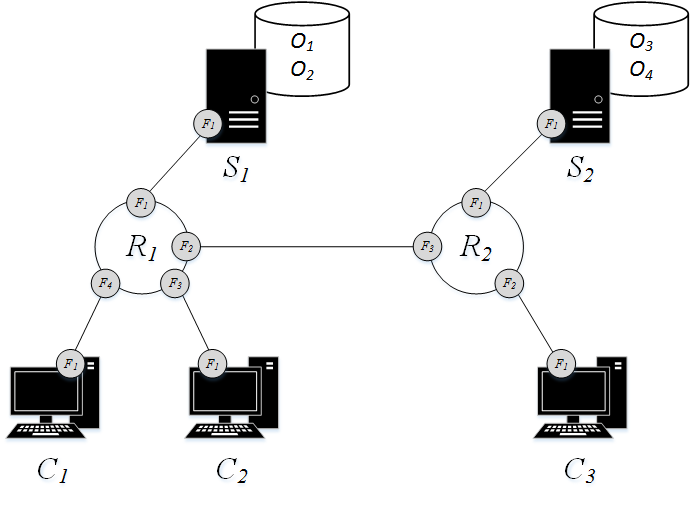
\includegraphics[width=0.30\textwidth]{figures/fib-topo.png}
    \cprotect\caption{Simple example of an NDN network topology.}
    \label{fig:fib-topo}

\end{figure}

\subsection{Endpoints}
\label{subsec:meth-endpoints}

In our model we consider two forms of endpoints: clients $C$ and servers $S$. 
Clients generate Interests for content, i.e. vectors in the form of \textbf{v} 
in~\ref{eq:signal}, while servers hold caches in which content objects persist 
and are always available.\shortvertbreak

The operation of servers is simple, basically consisting in mirroring the 
Interest signals received as input, according to the contents of their 
persistent CS:\shortvertbreak

\begin{algorithmic}[1]

\State \textbf{define} Server::mirror(\textbf{U}):
\State
    \State $\textbf{U}' \leftarrow \textbf{CS} \ \& \ \textbf{U}$ 
    \State
    \State $\textbf{Y}_h \leftarrow \begin{bmatrix} \textbf{0}^{|O|} \times {\textbf{1}^{|F|}}^{T} \\ \textbf{U}'(1:|O|,:) \end{bmatrix}$ 
    \State
    \State $F_{n,1:|F|,out} \leftarrow \textbf{Y}_h$

\end{algorithmic}\shortvertbreak

Clients generate Interest signals in a probabilistic fashion, e.g. according 
to some popularity distribution such as Zipf~\cite{6038471}. In our model, 
clients $C$ take (...).

\subsection{Cache Algorithms}
\label{subsec:meth-caching-algs}

\subsection{Network Topologies}
\label{subsec:meth-topologies}

We represent a network topology using a square matrix \textbf{T}, 
with dimension $|R|+|C|+|S|$. For representation purposes, we attribute an 
integer index to each one of the network nodes, and so each elements $(i,j)$ of the 
matrix corresponds to interconnections between network entities with indexes $i$ and $j$. The 
values at each $(i,j)$ position identify the \textbf{near end interface} of the 
connection, i.e. the interface at entity $i$. E.g. the matrix \textbf{T} shown 
in~\ref{eq:topo} encodes the topology shown in Figure~\ref{fig:fib-topo}. In this case, 
we attribute the integers 1 to 7 to the network entities, starting with the 
clients $C_1$ to $C_3$, then routers $R_1$ and $R_2$ and 
finally the servers $S_1$ and $S_2$.

\begin{equation}
\textbf{T} = \begin{bmatrix} 
                0 & 0 & 0 & 1 & 0 & 0 & 0               \\ 
                0 & 0 & 0 & 1 & 0 & 0 & 0               \\ 
                0 & 0 & 0 & 0 & 1 & 0 & 0               \\ 
                4 & 3 & 0 & 0 & 2 & 1 & 0               \\ 
                0 & 0 & 2 & 3 & 0 & 0 & 1               \\ 
                0 & 0 & 0 & 1 & 0 & 0 & 0               \\ 
                0 & 0 & 0 & 0 & 1 & 0 & 0               \\ \end{bmatrix}
    \label{eq:topo}
\end{equation}\shortvertbreak

\subsection{`Connecting the Dots'}
\label{subsec:meth-conn-dots}



\subsection{Implementation}
\label{subsec:meth-impl}

The NDN network model described above has been implemented in MATLAB\textsuperscript{\textregistered}, taking 
advantage of its Object Oriented Programming (OOP) capabilities. Most of 
the object types are independent of particular cache algorithms, nevertheless 
CS objects are defined as abstract classes, allowing for specific 
implementations of cache policies such as LRU, MRU and Random caching. The 
MATLAB\textsuperscript{\textregistered} 
code --- along with additional documentation --- is freely available 
at \url{github.com/adamiaonr/mtsp-project}.
